\section{Realisierung flache FSM}

\subsection{Mögliche Realisierungen von flachen FSMs}

\begin{outline}
    \1 Steuerkonstrukt (typischerweise mit \textbf{switch-case})
        \2 prozedural oder objektorientiert
    \1 Definition und Abarbeitung einer \textbf{Tabelle}
        \2 prozedural oder objektorientiert
    \1 \textbf{State Pattern} (Gang of Four, GoF)
        \2 nur objektorientiert
    \1 Generisch mit Templates
        \2 nur mit einer Sprache, die Templates unterstützt (z.B. C++)
\end{outline}

\vspace{0.2cm}

\textrightarrow\ Alle Varianten haben wie immer sowohl Vor- als auch Nachteile \\
\textrightarrow\ Bei allen Varianten sind auch Variationen vorhanden


\subsection{Realisieurng mit Steuerkonstrukt (prozedural in C)}

\subsubsection{State-Event-Diagram -- Up/Down-Counter}

\begin{center}
    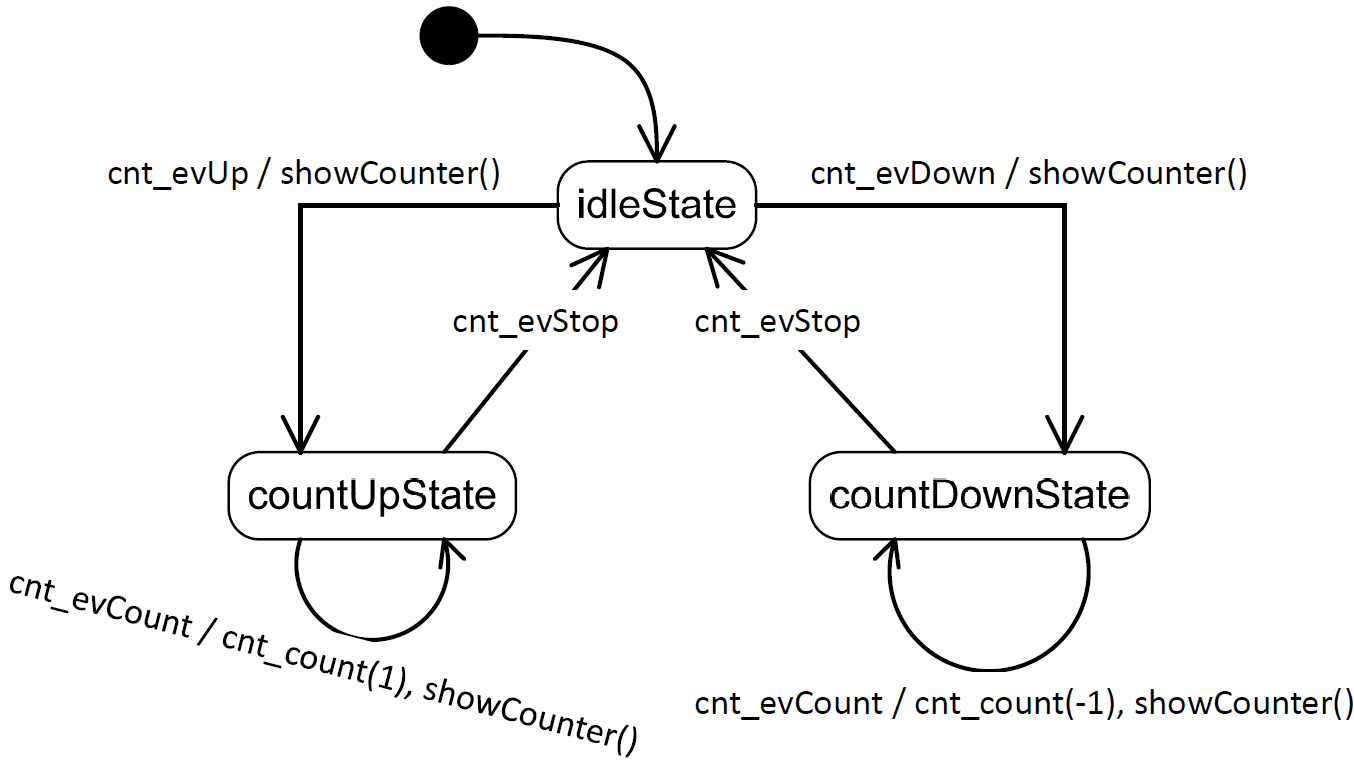
\includegraphics[width=0.7\columnwidth]{images/fsm_up-down-counter_diagramm_C.png}
\end{center}


\subsubsection{Implementation der Prozeduralen Realisierung in C}

\begin{outline}
    \1 \textbf{Ereignisse (events)}
        \2 Schnittstelle nach aussen \textrightarrow\ ändern Zustand der FSM
        \2 In enum definiert (\textbf{public}) \textrightarrow\ header-file
        \2 Einzelne Events und enum Bezeichnung enthalten \textbf{Unitkürzel} (hier: \mylstbox{cnt_})
    \1 \textbf{Zustände (states)}
        \2 In enum definiert (\textbf{nicht} public) \textrightarrow\ sourcecode-file
    \1 \textbf{Aktueller Zustand} wird in einer \textbf{statischen Varianlen} gehalten
    \1 Die FSM wird in \textbf{zwei Funktionen} implementiert
        \2 Initialiserungs-Funktion (hier: \mylstbox{void cnt_ctrlInit(int initValue)})
        \2 Prozess-Funktion (hier: \mylstbox{void cnt_ctrlProcess(cnt_Event e)}) \\
            \textrightarrow\ Zustände prüfen, Zustandsübergänge veranlassen
    \1 Anstossen einer FSM
        \2 Initialisierung in \lstinline|main|-Funktion
        \2 Überprüfung, welches Event aufgetreten ist meist in \mylstbox{do-while}-Schleife
\end{outline}


\subsubsection{Eigenschaften der Prozeduralen Realisierung in C}

\begin{outline}
    \1 Da aktueller Zustand eine statische Variable ist, kann es nur \textbf{eine einzige Instanz} der FSM geben
    \1 Bei mehreren Instanzen in C...
        \2 darf \mylstbox{currentState} nicht \mylstbox{static} sein und muss als Parameter mitgegenen werden,
            bzw. ein Pointer auf die jeweilige Variable
        \2 Zustands-enum muss in die Schnittstelle (header-file) oder es muss z.B. mit \mylstbox{void*} gearbeitet werden
    \1 In C ist \textbf{keine schöne Kapselung} der Attribute möglich (\mylstbox{currentState})
    \1 Funktion \mylstbox{cnt_ctrlProcess()} kann beliebig aufgerufen werden (periodischer Task, laufend, etc.)
    \1 Bei exponierten Funktionen / Definitionen muss in C ein Unitkürzel vorangestellt werden (hier: \mylstbox{cnt_})
\end{outline}


\example{Up/Down-Counter (prozedural in C)}

% TODO: \para environment not showing...?
% TODO: add keywords and stuff to listings setup

\begin{minipage}[t]{0.48\columnwidth}
    \para{Schnittstelle Counter in C} 
    \lstinputlisting{snippets/fsm_counter_C.h}
\end{minipage}
\hfill
\begin{minipage}[t]{0.48\columnwidth}
    \para{Implementation Counter in C} 
    \lstinputlisting{snippets/fsm_counter_C.c}
\end{minipage}


\para{Schnittstelle FSM in C} 
\lstinputlisting{snippets/fsm_counterCtrl_C.h} 

\para{Implementation FSM in C} 
\lstinputlisting{snippets/fsm_counterCtrl_C.c}

\para{Anstossen der FSM in C} 
\lstinputlisting{snippets/fsm_main_counterTest_C.c}



\subsection{Realisieurng mit Steuerkonstrukt (objektorientiert in C++)}

\subsubsection{State-Event-Diagram -- Up/Down-Counter}
\label{State-Event-Diagram -- Up/Down-Counter in CPP}

\begin{center}
    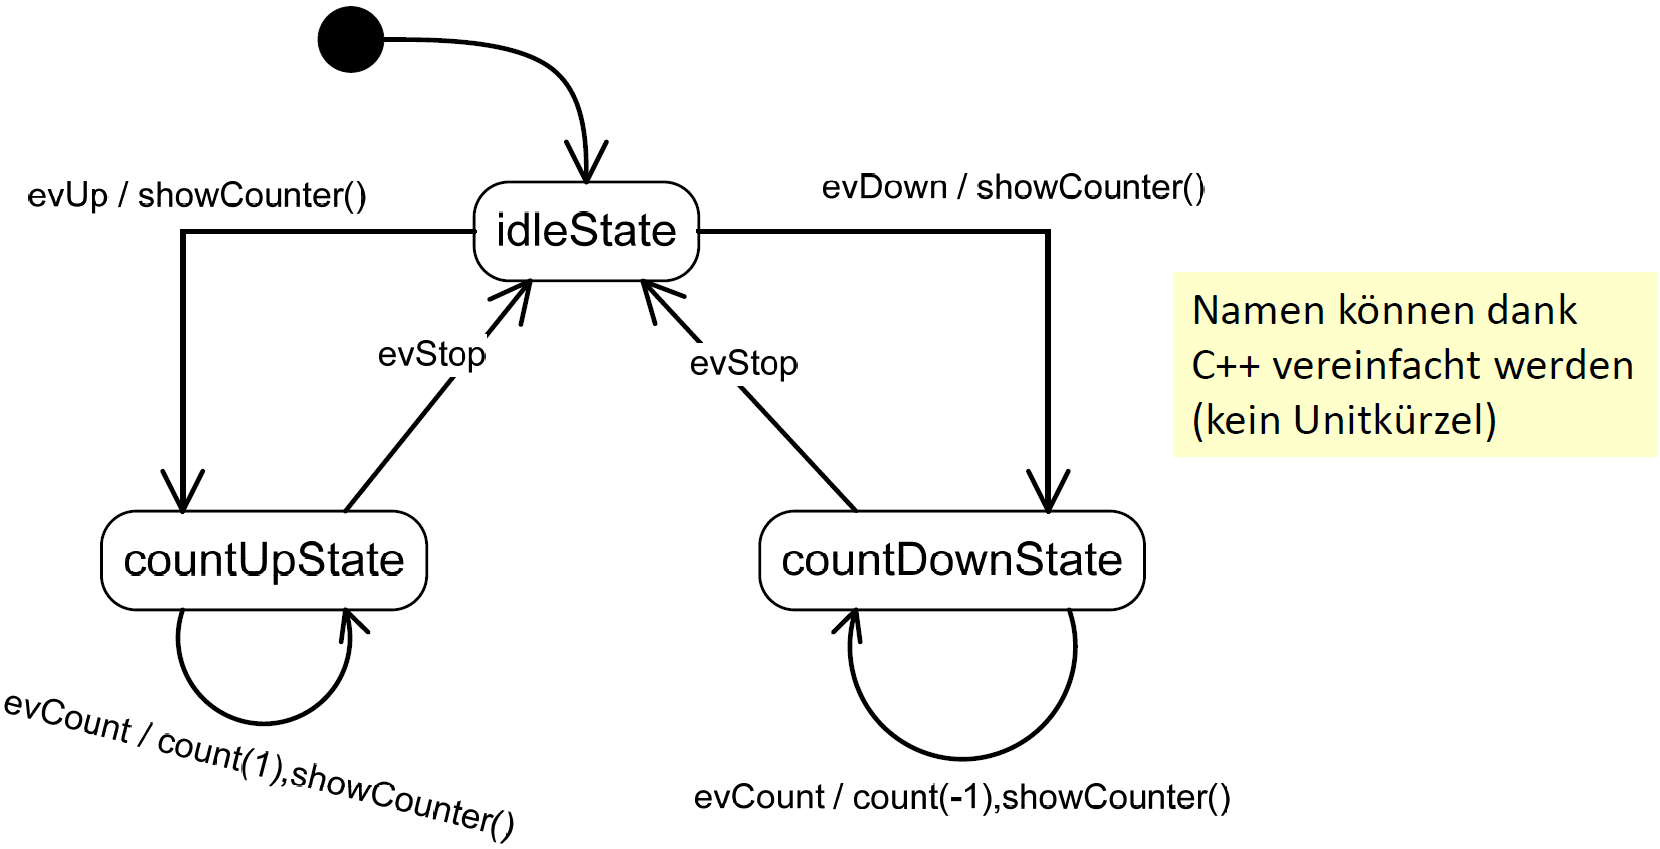
\includegraphics[width=0.7\columnwidth]{images/fsm_up-down-counter_diagramm_CPP.png}
\end{center}


\subsubsection{Zusammenhang der Klassen Counter und CounterCtrl}
\label{Zusammenhang der Klassen Counter und CounterCtrl}

\begin{center}
    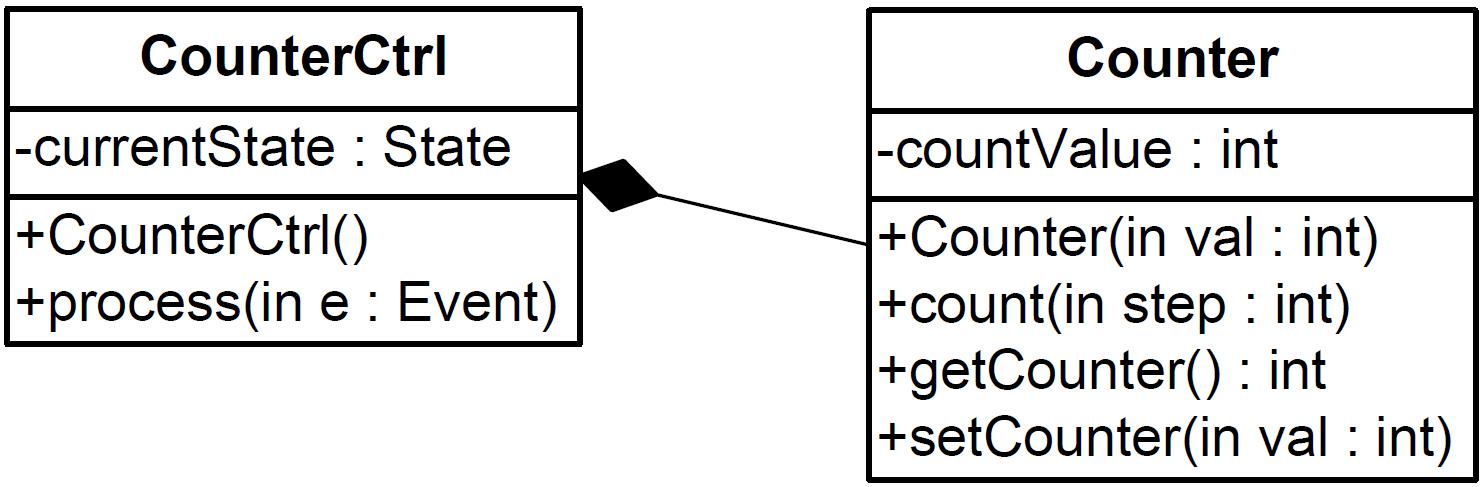
\includegraphics[width=0.7\columnwidth]{images/fsm_CPP_klassendiagramm.png}
\end{center}

\begin{outline}
    \1 Klasse \mylstbox{Counter} führt eigentliche Rechenaufgaben durch
        \2 ist bei \textbf{allen} (objektorientierten) Realiseurngsarten \textbf{identisch}
    \1 Klasse \mylstbox{CounterCtrl} ist FSM, welche Zugriff auf den Counter steuert 
\end{outline}

\textbf{ \textrightarrow\ Generell sollten Steuerung und Element, das gesteuert wird, getrennt werden!}


\subsubsection{Implementation der Prozeduralen Realisierung in C++}

\begin{outline}
    \1 \textbf{Ereignisse (events)}
        \2 Schnittstelle nach aussen \textrightarrow\ ändern Zustand der FSM
        \2 Im \textbf{public} Teil der Klasse als enum definiert
        \2 Keine Unitkürzel nötig
    \1 \textbf{Zustände (states)}
        \2 Im \textbf{private} Teil der Klasse als enum definiert \textrightarrow\ header-file
    \1 \textbf{Aktueller Zustand} \mylstbox{currentState} wird in \textbf{privatem Attribut} von \mylstbox{CounterCtrl} gehalten
    \1 Die FSM wird in \textbf{zwei Funktionen} implementiert
        \2 Kontruktor (hier: \mylstbox{CounterCtrl::CounterCtrl(int initValue=0)})
        \2 Prozess-Funktion (hier: \mylstbox{void CounterCtrl::process(CounterCtrl::Event e)}) \\
            \textrightarrow\ Zustände prüfen, Zustandsübergänge veranlassen
    \1 Anstossen einer FSM
        \2 Initialisierung in \lstinline|main|-Funktion
        \2 Überprüfung, welches Event aufgetreten ist meist in \mylstbox{do-while}-Schleife
\end{outline}


\example{Up/Down-Counter (prozedural in C++)}

% TODO: \para environment not showing...?
% TODO: add keywords and stuff to listings setup

\begin{minipage}[t]{0.44\columnwidth}
    \para{Schnitstelle Counter in C++} 
    \lstinputlisting{snippets/fsm_Counter_CPP.h}
\end{minipage}
\hfill
\begin{minipage}[t]{0.52\columnwidth}
    \para{Implementation Counter in C++} 
    \lstinputlisting{snippets/fsm_Counter_CPP.cpp}
\end{minipage}


\para{Schnittstelle FSM in C++} 
\lstinputlisting{snippets/fsm_CounterCtrl_CPP.h} 

\para{Implementation FSM in C++} 
\lstinputlisting{snippets/fsm_CounterCtrl_CPP.cpp}

\para{Anstossen der FSM} 
\lstinputlisting{snippets/fsm_main_counterTest_CPP.cpp}



\subsection{Realisierung mit Tabelle}

\subsubsection{State-Event-Diagram -- Up/Down-Counter}

Siehe Abschnitt \ref{State-Event-Diagram -- Up/Down-Counter in CPP}


\subsubsection{FSM in Tabellenform}

Das State-Event-Diagramm wird in eine Tabelle 'übersetzt'. \textbf{Jede Zeile der Tabelle entspricht einer Transition (Pfeil) im 
State-Event-Diagramm}

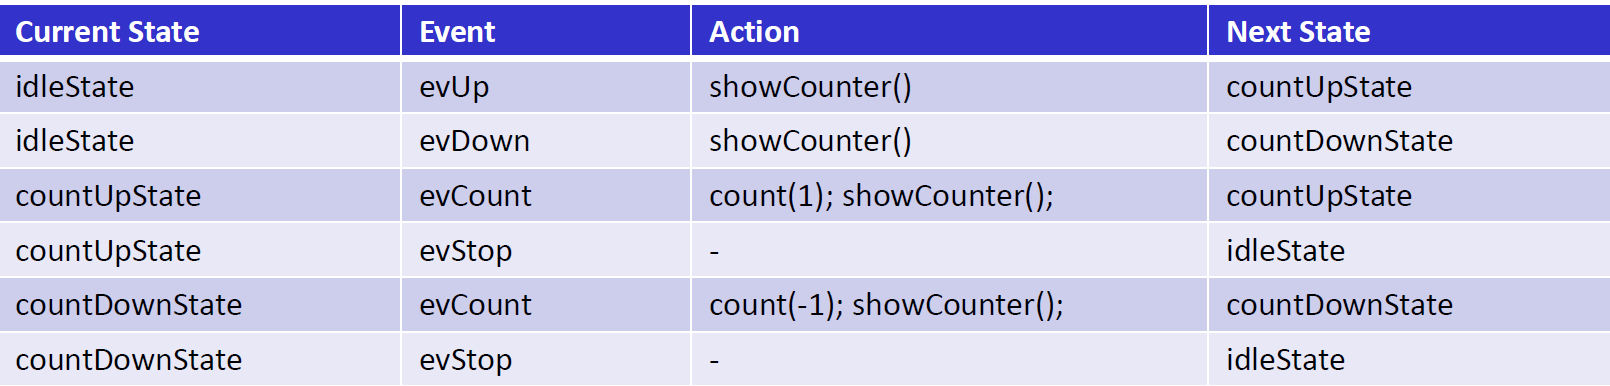
\includegraphics[width=\columnwidth]{images/fsm_tabelle.png}


\subsubsection{Implementation der Realisierung mittels Tabelle in C++}

\begin{outline}
    \1 Die ganze FSM ist in einer Tabelle gespeichert
    \1 \textbf{Aktionen} sind als \textbf{Funktion} implementiert, in der \textbf{Tabelle} steht der entsprichende \textbf{Funktionspointer} % CHECK: sind das Pointer auf Klassenelemente?
    \1 \textbf{Abarbeitung} der FSM erfolgt mittels \textbf{Execution Engine}, die in der Tabelle 'nachschaut', was zu tun ist
        \2 Execution Engine \textbf{ändert sich nicht}, wenn FSM geändert wird!
    \1 \textbf{Transition} wird als klasseninterner \mylstbox{struct} deklariert
        \2 enthält aktuellen Zustand, Event, Funktionspointer auf Aktionsmethode und nächsten Zustand
    \1 \textbf{FSM} wird als statischer, offener Array deklariert
        \2 Hier wird ganze FSM gespeichert
        \2 ein \mylstbox{struct} bildet konkret eine Zeile der Tabelle ab
\end{outline}


\subsubsection{Eigenschaften der Realisierung mittels Tabelle}

\begin{outline}
    \1 Die Tabelle kann prozedural oder \textbf{objektorientiert} implementiert werden
        \2 Objektorientierte Variante verwendet einzig die Datenkapselung (keine Vererbung, kein Polymorphismus)
        \2 Objektorientierte Variante ist klarer / schöner strukturiert
    \1 \textbf{Aktions-Funktionen} können \textbf{nicht inlined} werden, da ein Pointer auf die Funktionen verwendet wird
\end{outline}


\subsubsection{Tabelle vs. prozedural}

\begin{minipage}[t]{0.48\columnwidth}
    \raggedright
    \myul{\textbf{Gemeinsamkeiten}}
    
    \vspace{0.1cm}

    \begin{outline}
        \1 Testprogramm \mylstbox{counterTest.cpp}
        \1 Schnittstelle (public-Teil) von Klasse \mylstbox{CounterCtrl}
        \1 Gesamte Klasse \mylstbox{Counter}
    \end{outline}
\end{minipage}
\hfill
\begin{minipage}[t]{0.48\columnwidth}
    \raggedright
    \myul{\textbf{Unterschiede}}
    
    \vspace{0.1cm}

    \begin{outline}
        \1 private-Teil von Klasse \mylstbox{CounterCtrl} und Implementation davon
    \end{outline}
\end{minipage}


\example{Up/Down-Counter (mit Tabelle in C++)}

\para{Schnittstelle FSM in C++} 
\lstinputlisting{snippets/fsm_CounterCtrl_table_CPP.h} 

\para{Implementation FSM in C++} 
\lstinputlisting{snippets/fsm_CounterCtrl_table_CPP.cpp}


\subsection{Erweiterung der Realisierung mittels Tabellen}

\begin{itemize}
    \item Wenn der Zustandsübergang nicht durch einen Event, sondern eine \textbf{komplexere Prüfung (Event und Guard)} ausgelöst wird, 
        dann könnte der \textbf{Event-Eintrag} in der Tabelle durch einen weiteren \textbf{Funktionspointer} auf eine 
        \textbf{Checkfunktion ersetzt} werden.
    \item Ergänzung für die Behandlung von Entry- und Exit-Actions
\end{itemize}


\example{Up/Down-Counter (mit Checker-Tabelle in C++)}

\begin{outline}
    \1 Änderungen in \mylstbox{CounterCtrl.h} \textrightarrow\ siehe Beispiel-Code
    \1 Änderungen in \mylstbox{CounterCtrl.cpp}
        \2 checker-Funktionen müssen implementiert werden
        \2 In Tabelle steht statt Event die Adresse der checker-Funktion (analog zu action-Funktionen)
\end{outline}

\lstinputlisting{snippets/fsm_CounterCtrl_table_pChecker_CPP.h}

